\chapter{Algoritmos}
\label{Algoritmos}
\section{Algoritmo exato (\textit{Branch and Bound})}

% \textcolor{blue}{
% \textbf{Esta parte transcrevi diretamente do Texto de Kececioglu}\\
%  Na ultima seção nós obtemos um algoritmo que se aproxima do ótimo aplicando uma estratégia gulosa: de todas reversões, selecione uma que remove o máximo de breakpoints. Para obter um algoritmo que alcança o ótimo, nós usamos uma estratégia Branch and Bound: considerar todas reversões, e remover aquelas que não podem levar a uma solução ótima. No algoritmo nós mantemos 3 variáveis globais: $d*$  , um UpperBound dinâmico sobre o valor solução; $r*$, um vetor de reversões que ordena a permutação em $d*$  passos; e $r$, a série de reversões vigente sob consideração. No inicio inicializamos $d*$ e $r*$ com valores obtidos de um algoritmo UpperBound. O algoritmo que nós usamos é essencialmente guloso visando a frente profundidade fixa. 
%   Depois de um obter um Upper Bound no exploramos uma arvore de subproblemas depth-first. Cada invocação do Search corresponde a um nó da árvore e é rotulado com $\pi$, uma permutação para ser ordenada, e $d$, o número de arestas da raiz até o nó. Vetor $r$ é é mantido como uma pilha pelo Search, e trava as reversões sobre o caminho da raiz até o nó atual. Nós escolhemos uma estratégia depth-first para atravessar a árvore com isso usa uma quantidade de polinomial de espaço, mesmo quando a árvore é de tamanho exponencial pois o espaço, não o tempo, é o recurso limitante.
% }

O algoritmo de \textit{Branch and Bound} é um algoritmo exato utilizado para resolver problemas de otimização combinatória. Ele consiste na enumeração passo a passo de todos possíveis candidatos a compor o conjunto solução ótima (em nosso caso, as reversões), explorando todo o espaço de busca e construindo uma árvore de decisão, onde a cada nível abaixo da raiz temos decomposições do problema original. Sendo $\pi$ a raiz da árvore e $\rho_i$ uma reversão representada por uma aresta da árvore, logo $\pi \circ \rho_i$ é um nó filho de $\pi$. Podemos ver uma representação desta árvore na Figura \ref{DecisionTree}. 

% \FV{Usar índices na figura, tais como $\rho_1, \rho_2,$ etc.}

% \begin{figure}[h]

% \centering % para centralizarmos a figura
% 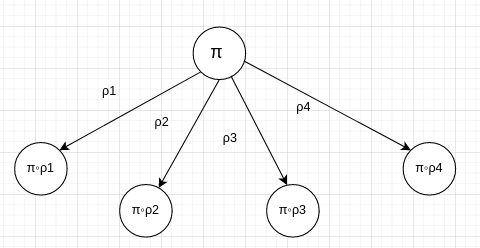
\includegraphics[width=8.0cm]{Imagens/decision_tree.png} % leia abaixo
% \caption{Representação da árvore de decisão do algoritmo exato.}
% \label{figura:Decision Tree}
% \end{figure}

\begin{figure}[h]
    \centering
    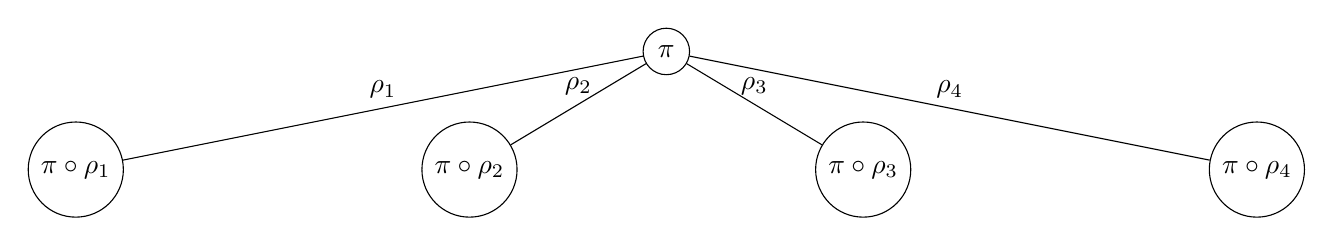
\begin{tikzpicture}[level/.style={sibling distance=50mm/#1}]
        \node [circle,draw] (z){$\pi$}
        child {node [circle,draw] (a) {$\pi \circ \rho_1$}
        edge from parent node [above] {$\rho_1$}}
        child {node [circle,draw] (b) {$\pi \circ \rho_2$}
        edge from parent node [above] {$\rho_2$}}
        child {node [circle,draw] (c) {$\pi \circ \rho_3$}
        edge from parent node [above] {$\rho_3$}}
        child {node [circle,draw] (d) {$\pi \circ \rho_4$}
        edge from parent node [above] {$\rho_4$}}
        ;

    \end{tikzpicture}
    \caption{Representação da árvore de decisão do algoritmo exato.}
    \label{DecisionTree}
\end{figure}

Para controlar o tamanho do espaço de busca da solução ótima, dois algoritmos são necessários, para computar os limitantes (\textit{Bounds}): o \textit{UpperBound}() e o \textit{LowerBound}(). Esses algoritmos calculam os valores que podem ser vistos como o intervalo onde a solução ótima se encontra e quanto mais refinados forem, menor será o tempo para processar a solução ótima. Diminuir o espaço de busca através destes algoritmos reflete na árvore de decisão como operações de poda, que diminuem a quantidade de nós, descartando conjuntos de soluções ruins até que apenas a solução ótima reste. Em nível de implementação, o algoritmo constrói uma lista com todas as reversões possíveis de uma permutação $\pi$ e as ordena em ordem decrescente em relação ao número de BPs removidos por cada reversão. Essa lista é percorrida e cada reversão $\rho_i$ é selecionada e aplicada sobre $\pi$. A quantidade de passos, isto é, a distância de um nó da árvore de decisão para a raiz, é incrementada em uma unidade e analisamos se o candidato $\rho_i$ selecionado está dentro dos limitantes correntes; caso esteja, uma chamada recursiva é realizada com $\pi \circ \rho_i$, no lugar de $\pi$; caso contrário, $\pi \circ \rho_i$ e todos os seus filhos na árvore são descartados. São usadas três variáveis globais que são mantidas em nosso algoritmo: um \textit{upperbound} dinâmico $d*$ contendo a quantidade de reversões de nossa solução, uma lista de reversões $r*$ que ordena a permutação em $d*$ passos e uma segunda lista de reversões $r$ com o conjunto de reversões atual sob análise.

Os limitantes são a chave do algoritmo exato, pois um limitante ruim ocasionaria em um aumento grande na quantidade de candidatos a serem analisados. Tendo isso em vista, os métodos escolhidos que calculam os limitantes, apesar de não serem os mais eficientes, são os mais intuitivos com um desempenho aceitável para a nossa proposta. O método para o cálculo do limitante superior que usamos é a maneira mais simples de gerar uma solução para nosso problema, descrita no algoritmo ingênuo na seção \ref{algoritmo_ingenuo}, que garante que nenhuma da sequências de reversões que forem encontradas posteriormente no algoritmo que realizam uma quantidade de passos superior seja considerada. Atualmente, nosso algoritmo que calcula o limitante superior é executado em tempo $\mathcal{O}{(n)}$. Para melhor conveniência, chamaremos o algoritmo ingênuo de \textit{Reversal Sort} e a figura \ref{figura:Execução do Reversal Sort} apresenta alguns passos de sua execução.


\begin{figure}[h]
% \caption{Exemplo \FV{Esta figura não é referenciada no texto e a legenda não diz nada.}}
% \RR{Corrigido}
\centering % para centralizarmos a figura
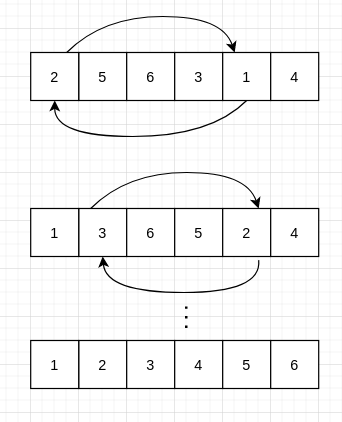
\includegraphics[width=5.8cm]{Imagens/reversalSort.png} % leia abaixo
\caption{Representação da execução do Reversal Sort.}
\label{figura:Execução do Reversal Sort}
\end{figure}


Em relação ao método que calcula o limitante inferior, sua função é devolver um valor para o melhor caso de execução possível, servindo como parâmetro de poda na árvore de decisão a cada iteração da lista de candidatos, ou seja, é calculado dinamicamente. Esse algoritmo é construído a partir da observação de que o melhor cenário é remover dois BPs com uma única reversão, como visto na seção \ref{limitante inferior}. A quantidade de passos de execução é a metade da quantidade de BPs, ou seja $\phi(\pi)/2$. Podemos calcular este limitante em tempo $\mathcal{O}{(n)}$, que é necessário para contar os BPs da permutação.  

A seguir é mostrado um pseudocódigo de nosso algoritmo \textit{Branch and Bound}.

\begin{comment}
A primeiro momento, uma permutação qualquer é dada como entrada na função UpperBound (limitante superior) que garantirá que nossa solução final não seja pior que a encontrada por este limitante. Com isso, as variáveis globais são atualizadas com o conjunto solução (quantidade de passos, e conjunto de reversões ),  encontrado pelo UpperBound, que poderá ser substituído caso encontremos uma solução melhor no processamento principal (função Branch and Bound). Na função principal do algoritmo recebemos a permutação de entrada junto com um 0 referente a quantidade de passos realizados até a solução final, após isso é verificado se a permutação de entrada já esta ordenada (se sim, não há nada a se fazer), e caso não esteja o algoritmo irá iterar em uma lista de reversões de ordem decrescente de $\Delta(\phi)$, a cada iteração a quantidade de passos é incrementada em 1 e a reversão atual é aplicada sobre a permutação. Se a quantidade de passos somada a um LowerBound (limitante inferior, que nos garante que a solução final não será melhor do que a encontrada pelo limitante) for menor que a quantidade passos obtida pelo UpperBound, nós iremos armazenar a reversão feita no conjunto solução e chamaremos a função principal recursivamente, agora com os parâmetros atualizados. Este processo principal é repetido até que a permutação esteja ordenada.
A saída do algoritmo é o conjunto solução contendo a quantidade de passos realizada pela solução ótima assim como as reversões que a compõem.
A seguir será demonstrado um pseudocódigo contendo o Algoritmo Branch and Bound proposto por e o pseudocódigo de nossa implementação do problema seguindo os parâmetros definidos pelo autor no artigo.\\
\end{comment}

\begin{algorithm}[H]
\label{Algoritmo Exato}
\SetAlgoLined
\textbf{Global: d*, r*[1..n], r[1..n]}\;
\textbf{\textit{Branch and Bound}($\pi$)}\;
  \quad  $d*, r*$ = \textbf{\textit{UpperBound}($\pi$)}\;
  \quad \textbf{Search($\pi$, $0$)}\;
  \quad \textbf{return $d*, r*$}\;
\textbf{Search($\pi$, $d$)}\; 
    \quad\If{$\pi$ é a identidade}{
    \quad \quad $d', r' = d, r$\;
    }
\quad \Else{
\For{ cada reversão $\rho$ em ordem decrescente de $\Delta\phi$}{
    \quad $d'$, $\pi'  = d + 1$, $\pi$ $\circ$ $\rho$\;
    \quad \If{$d'$ + \textbf{\textit{LowerBound}($\pi'$)} $<$ $d*$}{
        \quad \quad $r[d'] = \rho$\;
        \quad \quad \textbf{Search($\pi', d'$)}\;
    }
}
} 

\textbf{\textit{LowerBound}($\pi$)}\;
\quad \textbf{return $\lceil$ $\phi(\pi)/ 2$ $\rceil$}\;

\textbf{UpperBound($\pi$)}\;
\quad global $d*, r*$\;
\quad $d*, r* = $ \textbf{ReversalSort($\pi$)}

 \caption{Algoritmo Exato}
\end{algorithm}

% \FV{Esse algoritmo não é referenciado no texto, com um comando \textbackslash\!ref\{\}.}
% \RR{Corrigido}

\section{Algoritmo guloso (\textit{Greedy})}

% O Greedy Algorithm é um algoritmo de aproximação que utiliza uma estratégia gulosa. Algoritmos de aproximação são algoritmos que podem entregar uma solução próxima da ótima, ou seja, são como uma garantia do quão próximo estou de uma solução ótima.

O método guloso é um paradigma de construção de algoritmos que pode ser usado para resolução de problemas de otimização combinatória, consumindo tempo polinomial nos tamanhos de suas entradas, produzindo algoritmos intuitivos. Algoritmos gulosos buscam a cada iteração o melhor candidato local, ou seja, a opção que oferece o benefício mais óbvio e imediato para o problema, assim construindo uma solução passo a passo com cada candidato. Em nosso caso, a solução a ser construída é a menor quantidade de reversões necessárias para ordenar uma permutação. No primeiro momento, a solução mais intuitiva seria a de colocar cada elemento da permutação, um por um, em sua devida posição, executando $n-1$ passos no pior caso para uma permutação de $n$ elementos, como visto na seção \ref{algoritmo_ingenuo}. Porém, esta seria uma solução fraca, pois para alguns casos ela entrega uma resposta muito ruim. Um exemplo é a permutação $(0, n, n-1, \ldots , 2, 1, n+1)$ que poderia ser ordenada com uma única reversão, mas o algoritmo ingênuo usa $n-1$ reversões. A partir da definição de BP, uma solução melhor foi proposta por \cite{kececioglu1995exact}, na qual a cada iteração a reversão que remove o máximo de BPs possível é executada, e em casos de empate opta-se preferencialmente por aquelas que resultam em uma SD. 
% \FV{Usar rótulos e referências (comandos label e ref)}
% \FV{SD foi definido antes?} 
% \FV{O que é?}
% \FV{O que é uma ``resposta não satisfatória''?}

O algoritmo executa enquanto houver BP na permutação e a cada iteração ele busca uma reversão que remova o máximo de BPs possíveis. Nesta busca consideramos três casos, dois deles removem BPs e um caso que não remove nenhum mas ajusta a permutação. O primeiro caso é o  melhor cenário, remover dois BPs com uma única reversão. Caso não seja possível, o algoritmo busca uma reversão que remova apenas um BP com preferência em reversões em que seja deixada uma SD após a reversão. Esta informação adicional de utilizar \textit{strips} para construir uma solução é fruto de lemas e provas elaborados por \cite{kececioglu1995exact}, de onde extraímos dois principais resultados, sendo um teorema e um corolário:

\newtheorem{Theorem}{Teorema}
\begin{Theorem}
\label{teorema}
O algoritmo Greedy ordena todas permutações $\pi$ em no máximo $\phi(\pi)$ passos.
\end{Theorem}
\begin{prova}
Se $\pi$ possui uma SD, o algoritmo Guloso ordena $\pi$ em no máximo $\phi(\pi)$ reversões. Se $\pi$ não possui SD, qualquer reversão escolhida pelo \textit{Greedy} transformar $\pi$ em uma permutação $\pi'$ com SD tal que $\phi(\pi') \leq \phi(\pi)$. \textit{Greedy} ordena $\pi'$ em no máximo $\phi(\pi') - 1$ reversões, e que ordena $\pi$ em no máximo de $\phi(\pi)$ reversões.
Uma vez que $\phi(\pi) \leq n + 1$, \ref{teorema} implica que o algoritmo \textit{Greedy} finaliza em $\mathcal{O}(n)$ iterações e roda em tempo polinomial. Um algoritmo para problemas de otimização que roda em tempo polinomial e entrega uma solução cujo valor esta dentro de um fator $\varepsilon$ conhecido como algoritmo $\varepsilon-$aproximado por ordenação por reversões.
\end{prova}

\newtheorem{Corollary}{Corolário}
\begin{Corollary}
O algoritmo Greedy é uma 2-aproximação para ordenação por reversões.
\end{Corollary}
\begin{prova}
Escreva $Opt(\pi)$ como sendo o mínimo número de reversões para ordenar uma permutação $\pi$, e \textit{Greedy}$(\pi)$ para o número obtido pelo algoritmo \textit{Greedy}. Uma vez que a solução deve remover todos os BPs e qualquer reversão pode remover no máximo dois BPS, temos que
\[ Opt(\pi) \ \ge \ \frac{1}{2}\phi(\pi) \ \ge \ \frac{1}{2}\textit{Greedy}(\pi).\] \\

Ou seja, temos a garantia de que no pior caso não executaremos mais que o dobro do numero de reversões da solução $Opt$.
\end{prova}

% Ou seja, a solução $Opt$ pode ser até duas vezes menor que a quantidade de BP ou que a resposta do algoritmo Greedy. 

O algoritmo \textit{Greedy} beneficia-se deles pois aumenta a garantia de que teremos êxito na remoção de um BP não só no passo atual como também em um passo futuro. Não sendo possível remover um BP que deixa uma SD, faremos apenas a remoção de um BP, mas se nenhum dos casos anteriores forem possíveis de serem executados, um passo de ajuste que não remove BP algum é executado e reorganiza a permutação, abrindo caminho para reversões que removem BPs. Em nenhum momento podemos executar uma reversão que aumenta a quantidade de BPs, pois uma reversão como essa nunca fará parte da solução com menor quantidade de reversões. Isso comprometeria os resultados do algoritmo, além de tornar o laço externo um \textit{loop} infinito. A saída do algoritmo consiste na quantidade de reversões aplicadas na permutação original até alcançar a identidade, além do conjunto de reversões aplicadas, nosso algoritmo \textit{Greedy} possui complexidade de $\mathcal{O}(n^2)$.

A seguir é mostrado um pseudocódigo de nosso Algoritmo \textit{Greedy}.


\begin{algorithm}[H]
\label{Algoritmo Greedy}
\SetAlgoLined
\textbf{Greedy($\pi$)}\;
 $i = 0$\;
 \While{$\pi$ contém BP}{
  $i = i + 1$\;
  Faça uma reversão $\rho$ em $\pi$ que remova o máximo de BP. Se o máximo for 1, priorize reversões que deixam uma sub-cadeia decrescente\;
  $\pi$ = $\pi \circ \rho$\;
 }
 \textbf{return} $i \  \rho_1, \rho_2, \rho_3 ...$\;
 \caption{Algoritmo \textit{Greedy}}
\end{algorithm}

% Alguns Lemas acompanham o desenvolvimento de nosso algoritmo Greedy, e nos são fundamentais para garantir 
% \begin{lema}
% \label{lema3}
% O algoritmo Greedy ordena uma permutação $\pi$ com uma SD em no máximo $\phi(\pi)-1$ reversões.
% %   \textcolor{red}{To Do}
% \end{lema}
% \begin{prova}
% A prova é por indução sobre $\phi(\pi)$. Se $\pi$ possui uma SD, $\phi(\pi)$ $\ge$ 2. Quando $\phi(\pi) = 2$, $\pi$ possui uma única reversão $\rho$ que remove os 2 BP e ordena $\pi$, assim  o \textit{Greedy} irá escolhe-lá.

% Suponha que o lema seja válido para todas permutações $\pi'$ com menos de que $\phi(\pi)$ BP. Desde que $\pi$ possua uma SD, por \ref{lema1} há uma reversão $\rho$ que remove ao menos um BP. Assim o primeiro passo do Greedy transformará uma permutação $\pi$ em $\pi'$ com no máximo $\phi(\pi) - 1$ BP. Se $\pi'$ possui uma SD, Greedy ordenará em no máximo $\phi(\pi) - 2$ por hipótese de indução na qual $\pi$ é ordenado em no máximo $\phi(\pi) - 1$ reversões.
%  Agora consideramos que $\pi'$ não possua SD. Nós argumentamos que $\phi(\pi') = \phi(pi) - 2$. Por suposição $\phi(\pi') = \phi(pi)-1$, a uma única outra possibilidade. Desde que o \textit{Greedy} escolhe a reverwsão que remove o máximo de BP, não deve haver reversão que remova dois BP. Em outras palavras, toda reversão que remover um BP, remove unicamente um BP. 

% \FV{Finalizar a prova}
% \end{prova}

% \begin{lema}
% \label{lema3}
% O algoritmo Greedy ordena uma permutação $\pi$ com uma SD em no máximo $\phi(\pi)-1$ reversões.
% %   \textcolor{red}{To Do}
% \end{lema}
% \begin{prova}
% A prova é por indução sobre $\phi(\pi)$. Se $\pi$ possui uma SD, $\phi(\pi)$ $\ge$ 2. Quando $\phi(\pi) = 2$, $\pi$ possui uma única reversão $\rho$ que remove os 2 BP e ordena $\pi$, assim  o \textit{Greedy} irá escolhe-lá.

% Suponha que o lema seja válido para todas permutações $\pi'$ com menos de que $\phi(\pi)$. Desde que $\pi$ possua uma SD, por \ref{lema1} há uma reversão que remove ao menos um BP. Assim o primeiro passo do Greedy transformará uma permutação $\pi$ em $\pi'$ com no máximo $\phi(\pi) - 1$ BP. Se $\pi'$ possui uma SD Greedy ordenará em no máximo $\phi(\pi) - 2$ por hipótese de indução que ordena $\pi$ em no máximo 1 reversão.

% % \FV{Finalizar a prova}
% \end{prova}

% \newtheorem{Theorem}{Teorema}
% \begin{Theorem}
% O algoritmo Greedy ordena toda permutação $\pi$ em no máximo $\phi(\pi)$ passos.
%   \textcolor{red}{To Do}
% \end{Theorem}
% \begin{prova}
% Se $\pi$ possui uma SD, pelo \ref{lema3}, o algoritmo Guloso ordena $\pi$ em no máximo $\ $
% \end{prova}

% \newtheorem{Corollary}{Corolário}
% \begin{Corollary}
% O algoritmo Greedy é uma 2-aproximação para ordenação por reversões.
% \end{Corollary}
% \begin{prova}
% Escreva $Opt(\pi)$ como sendo o mínimo número de reversões para ordenar uma permutação $\pi$, e \textit{Greedy}$(\pi)$ para o número obtido pelo algoritmo \textit{Greedy}. Uma vez que a solução deve remover todos os BPs e uma reversão remove no máximo dois BPS, temos que
% \[ Opt(\pi) \ \ge \ \frac{1}{2} \ \ge \ \frac{1}{2}\textit{Greedy}(\pi).\]
% \end{prova}

\begin{comment}
\begin{algorithm}[H]
\SetAlgoLined
\textbf{Algoritmo \textit{Greedy}($\pi$)}\;
 i  = 0\;
 \While{$\pi$ contém BP}{
  i = i + 1\;
  \While{1 até n}{
  Procure uma 2-reversao}
\While{1 até n}{
  Procure uma 1-reversao-SD}
 \While{1 até n}{
 Procure uma 1-reversao}
  \While{1 até n}{
 Procure uma 0-reversao}
$\rho = n$-reversao\;
  $\pi$ = $\pi \circ \rho$\;
 }
 \textbf{return} $i \  \rho_1, \rho_2, \rho_3 ...$.\;
 \caption{Algoritmo aproximado}
\end{algorithm}
\end{comment}

% O consumo de tempo deste algoritmo é o seguinte. Observe que o laço principal (mais externo) consome tempo $\mathcal{O}{(\phi(\pi))}$ no pior caso e cada passo interno consumo tempo $\mathcal{O}{(n)}$. Como um todo, o consumo de tempo pode ser simplificado para $\mathcal{O}{(n^{2})}$ e o espaço consumido é $\mathcal{O}{(n)}$. Um algoritmo aproximado se fez necessário nos estudos de \cite{kececioglu1995exact}, pois o \textit{Branch and Bound} possui a amplitude de testes limitada por seu consumo excessivo de tempo. Apesar de não devolver a resposta exata, o algoritmo \textit{Greedy} tem melhor desempenho para permutações extensas, devolvendo um resultado satisfatório em um tempo de execução mais aceitável. 